\documentclass[a4paper]{article}
\usepackage{amsfonts}
\usepackage{amsmath}
\usepackage{amssymb}
\usepackage{graphicx}     

\begin{document}
  
\noindent \large Auteur: Sabawoon Enayat      \\
\noindent \large Studierichting: Informatica  \\
\noindent \large Oefeningenreeks 3E nr. 11 \\

\newcommand{\Bgcos}{\operatorname{Bgcos}}

\medskip

\normalsize

Opgave: $l(x) = \dfrac{k\cos x}{d^2}$\\

$\overset{SOS}{\Rightarrow } d = \dfrac{a}{\sin x}$\\

$l(x) = \dfrac{k\cos x}{\left(\dfrac{a}{\sin x}\right)^2} = \dfrac{k\sin^2 x \cos x}{a^2 }$\\

$l'(x) = \dfrac{k}{a^2}\left(\sin 2x \cos x - \sin^3 x\right) = \dfrac{k}{a^2}\left(2\sin x \cos^2 x - \sin^3 x\right) = \dfrac{k}{a^2}\sin x\left(2\cos^2 x - \sin^2 x\right)$\\

$l'(x) = 0 \Rightarrow \dfrac{k}{a^2}\sin x\left(2\cos^2 x - \sin^2 x\right) = 0$\\

$\Rightarrow k = 0$ of $\sin x = 0$ of $2\cos^2 x - \sin^2 x = 0$\\

$\Rightarrow k$ gegeven\\

$\Rightarrow \sin x = 0 \Rightarrow x = 2m\pi$ of $x = \pi + 2m\pi$ met $\pi \in \mathbb{Z} \Rightarrow L $ naar boven of onder\\

$\Rightarrow 2\cos^2 x - \sin^2 x = 0 \Rightarrow 2\cos^2 x - (1 - \cos^2 x) = 0 \Rightarrow 2\cos^2 x - 1 + \cos^2 x = 0$\\

$\Rightarrow 3\cos^2 x = 1 \Rightarrow \cos^2 x = \dfrac{1}{3} \Rightarrow \cos x = \sqrt{\dfrac{1}{3}} \Rightarrow \cos x = \pm \dfrac{\sqrt{3}}{3}$

$\Rightarrow \cos x = -\dfrac{\sqrt{3}}{3} \Rightarrow$ niet mogelijk\\

$\Rightarrow \cos x = \dfrac{\sqrt{3}}{3} \Rightarrow x = \Bgcos \dfrac{\sqrt{3}}{3} + 2m\pi$ met $m \in \mathbb{Z}$\\

mogelijke $x$-waarden: $x = \Bgcos \dfrac{\sqrt{3}}{3} + 2m\pi$ met $m \in \mathbb{Z}$\\

$l''(x) = \dfrac{k}{a^2}\left(\left(2\cos x \cos 2x - \sin x \sin 2x\right) - \left(3\sin^2 x \cos x\right)\right) = \dfrac{k}{a^2}\left(\cos x\left(2\cos 2x - 3\sin^2 x\right) - \sin x\sin 2x\right)$\\

$l''\left(\Bgcos \dfrac{\sqrt{3}}{3}\right) \approx -0,57073\dfrac{k}{a^2} < 0 \Rightarrow$ maximum\\

$d^2 = a^2 + h^2 \Rightarrow h^2 = d^2 - a^2 \Rightarrow h = \sqrt{d^2 - a^2} = \sqrt{\left(\dfrac{a}{\sin x}\right)^2 - a^2}$\\

$h = \sqrt{\dfrac{a^2}{\sin^2 x} - a^2} = \sqrt{\dfrac{a^2 - a^2 \sin^2 x}{\sin^2 x}} = \sqrt{\dfrac{a^2 (1 - \sin^2 x)}{\sin^2 x}} = \sqrt{\dfrac{a^2 \cos^2 x}{\sin^2 x}}$\\

$h = \sqrt{a^2 \cot^2 x} = a\cot x = a\cot\left(\Bgcos \dfrac{\sqrt{3}}{3}\right) = a\dfrac{\cos\left(\Bgcos \dfrac{\sqrt{3}}{3}\right)}{\sin\left(\Bgcos \dfrac{\sqrt{3}}{3}\right)}$\\

$h = a\dfrac{\dfrac{\sqrt{3}}{3}}{\sqrt{1 - \dfrac{\sqrt{3}^2}{3^2}}} = a\dfrac{\dfrac{\sqrt{3}}{3}}{\sqrt{1 - \dfrac{1}{3}}} = a\dfrac{\dfrac{\sqrt{3}}{3}}{\dfrac{\sqrt{2}}{\sqrt{3}}} = a\dfrac{\sqrt{3}}{3}\dfrac{\sqrt{3}}{\sqrt{2}} = a\dfrac{3}{3\sqrt{2}} = \dfrac{a}{\sqrt{2}}$\\

\begin{figure}[h]
	\centering
	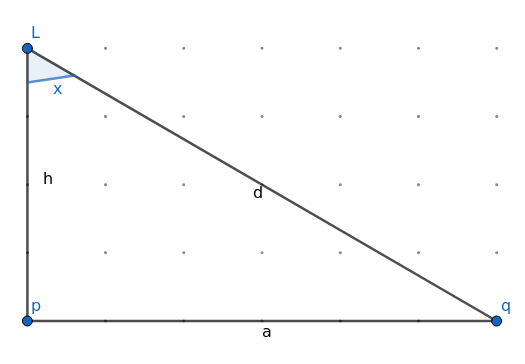
\includegraphics[width=10cm]{3E-11-sabawoon.enayat.INF.png}
\end{figure}

\begin{thebibliography}{999}
%\bibitem{a} Referentie
\end{thebibliography}
\end{document} 
